\section{Merging permutations}
\label{section:Merging permutations}

We are back to merging permutations. 
We show how to transform matching merges to permutation merges.

\begin{proposition}
  \label{proposition:3-merge permutation is NP-complete}
  \textsc{$3$-Merge Permutation} is \NP-complete.
\end{proposition}

\begin{proof}
  We reduce from \textsc{$3$-Merge Matching} (Proposition~\ref{proposition:3-Linear Graph Coloring is NP-complete}).
  Let $\mathcal{M}^{0}$, $\mathcal{M}^{1}$, $\mathcal{M}^{2}$, $\mathcal{M}^{3}$ be four matchings. 
  Write $\mathcal{M}^{i} = (V^i, E^i)$,
  $n_i = |V^i|$ and $m_i = |E^i|$ for $0 \leq i \leq 3$.
  We show how to construct permutations $\pi^0$, $\pi^1$, $\pi^2$ and $\pi^3$ such that
  the matching $\mathcal{M}^{0}$ is a merge of the matchings $\mathcal{M}^{1}$, $\mathcal{M}^{2}$ and $\mathcal{M}^{3}$
  if and only if
  the permutation $\pi^0$ is a merge of the permutations $\pi^0$, $\pi^2$ and $\pi^3$.

  Define $N = 8m_0 + 1$.
  We first associate the permutation $\pi^0$ to the matching $\mathcal{M}^{0}$.
  Write $V^0 = \{v^0_i : 1 \leq i \leq n_0\}$ and
  $E^0 = \{e^0_k : 1 \leq k \leq m_0\}$, where the edges are sorted according to their minimum vertex.
  \begin{alignat*}{3}
    &\forall i \in V_0,
    &\quad&
    \pi[i] &=&\; \BOXED{i fst}{4i} \quad \BOXED{i snd}{4i-3} \\ 
    &\forall e^0_k = (i,j) \in E_0,
    &\quad&
    \pi[e^0_k] &=&\; \BOXED{e fst}{2i} \quad \BOXED{e i}{3N_0 + 2m_0 + 4(i-1) + 2} \quad \BOXED{e j}{3N_0 + 2m_0 +4(j-1) + 3} \quad \BOXED{e snd}{2i - 1} \\
    \intertext{We have two groups of three separators 
    ($\text{sep}^{k}_{l}$, $1 \leq k \leq 2$ and $1 \leq l \leq 3$) that are defined as follows:}
    &&\quad&
    \pi[\text{sep}^{1}_{1}] &=&\; \BOXED{sep 1 1 1}{2N_0 + 2m_0 + 1} \quad \BOXED{sep 1 1 2}{2N_0 + 2m_0 + 2} \quad \dots \quad \BOXED{sep 1 1 N0}{2N_0 + 2m_0 + N_0} \\ 
    &&\quad&
    \pi[\text{sep}^{1}_{2}] &=&\; \BOXED{sep 1 2 1}{N_0 + 2m_0 + 1} \quad \BOXED{sep 1 2 2}{N_0 + 2m_0 + 2} \quad \dots \quad \BOXED{sep 1 2 N0}{N_0 + 2m_0 + N_0} \\ 
    &&\quad&
    \pi[\text{sep}^{1}_{3}] &=&\; \BOXED{sep 1 3 1}{2m_0 + 1} \quad \BOXED{sep 1 3 2}{2m_0 + 2} \quad \dots \quad \BOXED{sep 1 3 N0}{2m_0 + N_0} \\ 
    &&\quad&
    \pi[\text{sep}^{2}_{1}] &=&\; \BOXED{sep 2 1 1}{5N_0 + 2m_0 + 1} \quad \BOXED{sep 2 1 2}{5N_0 + 2m_0 + 2} \quad \dots \quad \BOXED{sep 2 1 N0}{5N_0 + 2m_0 + N_0} \\ 
    &&\quad&
    \pi[\text{sep}^{2}_{2}] &=&\; \BOXED{sep 2 2 1}{4N_0 + 2m_0 + 1} \quad \BOXED{sep 2 2 2}{4N_0 + 2m_0 + 2} \quad \dots \quad \BOXED{sep 2 2 N0}{4N_0 + 2m_0 + N_0} \\ 
    &&\quad&
    \pi[\text{sep}^{2}_{3}] &=&\; \BOXED{sep 2 3 1}{3N_0 + 2m_0 + 1} \quad \BOXED{sep 2 3 2}{3N_0 + 2m_0 + 2} \quad \dots \quad \BOXED{sep 2 3 N0}{3N_0 + 2m_0 + N_0}\text{.}
    \intertext{Define}
    &&\quad&
    \pi[V_0] &=&\; \pi[1] \; \pi[2] \; \dots \; \pi[|V_0|] \\
    &&\quad&
    \pi[E_0] &=&\; \pi[e^0_1] \; \pi[e^0_2] \; \dots \; \pi[e^0_{|E_0|}] \\
    &&\quad&
    \pi[\text{sep}^{1}] &=&\; \pi[\text{sep}^{1}_{1}] \; \pi[\text{sep}^{1}_{2}] \; \pi[\text{sep}^{1}_{3}] \\
    &&\quad&
    \pi_[\text{sep}^{2}] &=&\; \pi[\text{sep}^{2}_{1}] \; \pi[\text{sep}^{2}_{2}] \; \pi[\text{sep}^{2}_{3}]\text{.}
  \end{alignat*}
  The permutations $\pi^0$ is defined as follows:
  $$
  \pi^0 = \pi[V_0] \; \pi[\text{sep}^{1}] \; \pi[E_0] \; \pi[\text{sep}^{2}]\text{.}
  $$
  In other words,
  $\pi[V_0]$ is the direct sum of $2m_0$ decreasing permutations
  that are all order-isomorphic to $21$,
  $\pi[E_0]$ is the direct sum of $m_0$ permutations that are all
  order-isomorphic to $2341$, and
  both $\pi[\text{sep}^{1}]$ and $\pi[\text{sep}^{2}]$ are the skew sums
  of $k$ permutations that are all order isomorphic to $12 \dots k$.
  Viewed as a permutation matrix, the permutation $\pi^0$ has the following general shape:
  $$
    A(\pi^0) = 
    \begin{pmatrix}
      \pi[V_0] & 0                    & \pi[E_0] & 0 \\
      0        & 0                    & 0        & \pi[\text{sep}^{2}] \\
      0        & \pi[\text{sep}^{1}]  & 0        & 0  \\
      0        & 0                    & \pi[E_0] & 0 
    \end{pmatrix}\text{.}
  $$

  \begin{figure}
  \centering
  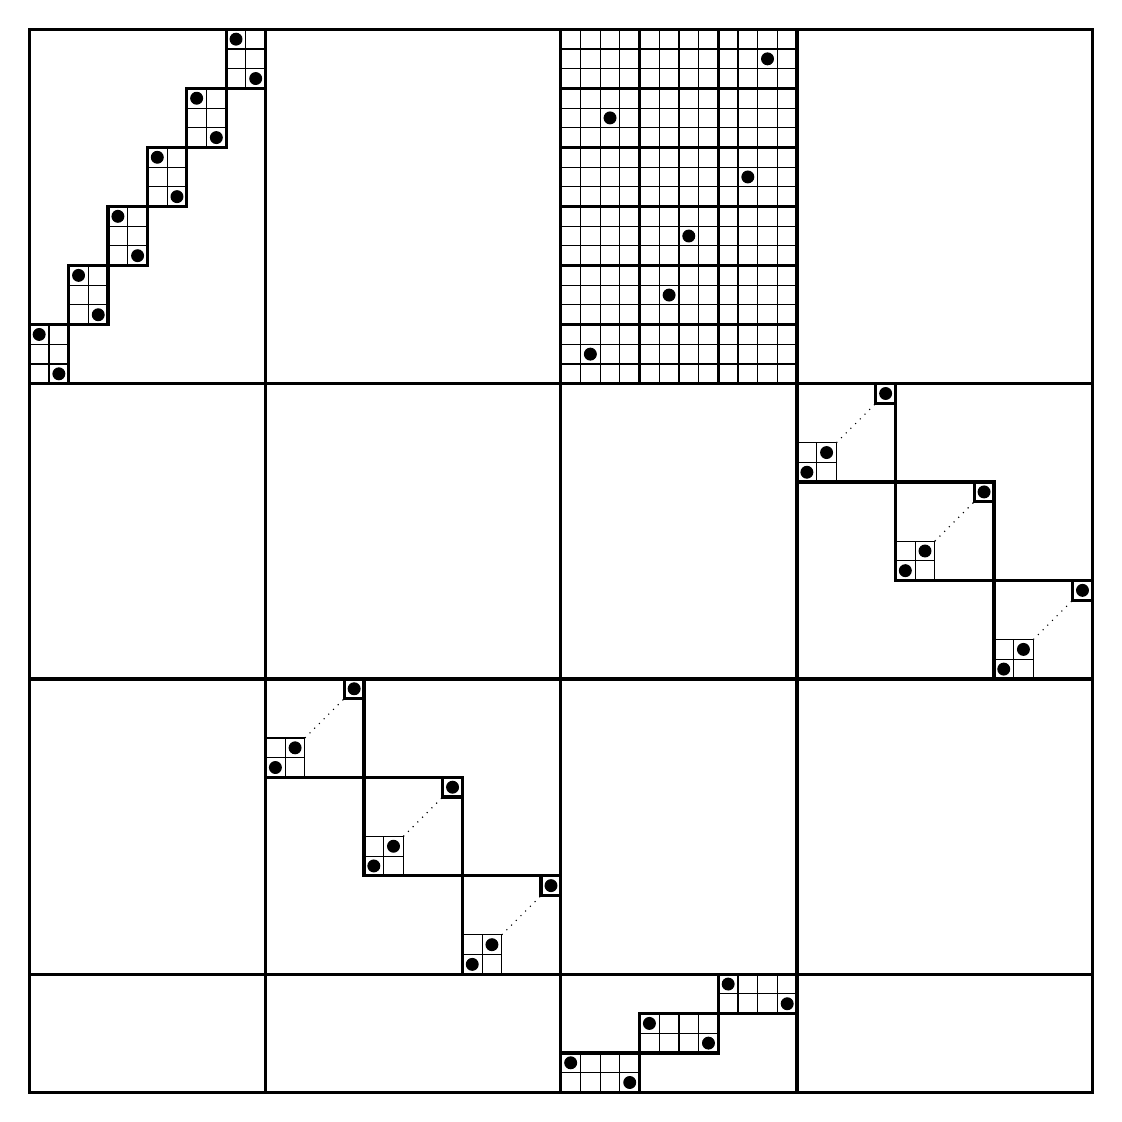
\begin{tikzpicture}
  [
    scale=.25,
  ]
  
  % grid
  \draw [step=1.0, black, very thick] (0,0) rectangle (54,54);
  \draw [step=1.0, black, very thick] (12,0) -- (12,54);
  \draw [step=1.0, black, very thick] (27,0) -- (27,54);
  \draw [step=1.0, black, very thick] (39,0) -- (39,54);
  \draw [step=1.0, black, very thick] (0,6) -- (54,6);
  \draw [step=1.0, black, very thick] (0,21) -- (54,21);
  \draw [step=1.0, black, very thick] (0,36) -- (54,36);

  % vertices
  \def\y{36}
  \foreach \i in {1,2,...,6} {
    \draw [step=1.0, black] (2*\i - 2, \y + 3*\i - 3) grid (2*\i, \y + 3*\i);
    \draw [black, very thick] (2*\i - 2, \y + 3*\i - 3) rectangle (2*\i, \y + 3*\i);
    \draw [fill=black] (2*\i - 1.5, \y + 3*\i - .5) circle (0.3);
    \draw [fill=black] (2*\i - .5, \y - 2 + 3*\i - .5) circle (0.3);
  }
  
  % edges
  \draw [step=1.0, black] (27,36) grid (39, 54);
  \draw [black, very thick] (27,36) rectangle (39, 54);
  \foreach \k/\i/\j in {1/1/5,2/2/3,3/4/6} {
    \draw [step=1.0, black] (4*\k + 23, 2*\k - 2) grid (4*\k + 27, 2*\k);
    \draw [black, very thick] (4*\k + 23, 2*\k - 2) rectangle (4*\k + 27, 2*\k);
    \draw [fill=black] (4*\k + 23 + 1 - .5, 2*\k - .5) circle (0.3);
    \draw [fill=black] (4*\k + 23 + 4 - .5, 2*\k - 1 - .5) circle (0.3);
    \draw [fill=black] (4*\k + 23 + 2 - .5, 36 + 3*\i - 1 - .5) circle (0.3);
    \draw [fill=black] (4*\k + 23 + 3 - .5, 36 + 3*\j - 1 - .5) circle (0.3);
  }
  % horizontal
  \draw [black, very thick] (31, 36) -- (31, 54);
  \draw [black, very thick] (35, 36) -- (35, 54);
  % vertical
  \draw [black, very thick] (27, 39) -- (39, 39);
  \draw [black, very thick] (27, 42) -- (39, 42);
  \draw [black, very thick] (27, 45) -- (39, 45);
  \draw [black, very thick] (27, 48) -- (39, 48);
  \draw [black, very thick] (27, 51) -- (39, 51);


  % separators 2
  \def\x{39}
  \def\y{31}
  \foreach \i in {1,2,3} {
    \def\xs2{\x + 5*\i - 5}
    \def\ys2{\y - 5*\i + 5}
    \draw [black, very thick] (\xs2, \ys2) rectangle (\xs2 + 5, \ys2 + 5);
    \draw [step=1.0, black] (\xs2, \ys2) grid (\xs2 + 2, \ys2 + 2);
    \draw [dotted] (\xs2 + 2, \ys2 + 2) -- (\xs2 + 4, \ys2 + 4);
    \draw [black, very thick] (\xs2 + 4, \ys2 + 4) rectangle (\xs2 + 5, \ys2 + 5);
    \draw [fill=black] (\xs2 + .5, \ys2 + .5) circle (0.3);
    \draw [fill=black] (\xs2 + 1.5, \ys2 + 1.5) circle (0.3);
    \draw [fill=black] (\xs2 + 4.5, \ys2 + 4.5) circle (0.3);
  }

  % separators 1
  \def\x{12}
  \def\y{16}
  \foreach \i in {1,2,3} {
    \def\xs2{\x + 5*\i - 5}
    \def\ys2{\y - 5*\i + 5}
    \draw [black, very thick] (\xs2, \ys2) rectangle (\xs2 + 5, \ys2 + 5);
    \draw [step=1.0, black] (\xs2, \ys2) grid (\xs2 + 2, \ys2 + 2);
    \draw [dotted] (\xs2 + 2, \ys2 + 2) -- (\xs2 + 4, \ys2 + 4);
    \draw [black, very thick] (\xs2 + 4, \ys2 + 4) rectangle (\xs2 + 5, \ys2 + 5);
    \draw [fill=black] (\xs2 + .5, \ys2 + .5) circle (0.3);
    \draw [fill=black] (\xs2 + 1.5, \ys2 + 1.5) circle (0.3);
    \draw [fill=black] (\xs2 + 4.5, \ys2 + 4.5) circle (0.3);
  }

  \end{tikzpicture}
\end{figure}

  A simplified representation of the permutation $\pi$ is given in
  Figure~\ref{fig:NP2:bird eye view pi}.
  A schematic representation of $\pi(\text{Sep}_1)$ and $\pi(\text{Sep}_2)$
  is given in Figure~\ref{fig:NP2:separators}, where the offset is $O=2n$ for
  $\pi(\text{Sep}_1)$ and $O=2n+kN$ for $\pi(\text{Sep}_2)$.
  A zoom of $\pi(E)$ is given in Figure~\ref{fig:NP2:connection zoom}.

  For example, referring Figure~\ref{fig:3-Linear-Graph Coloring} ($k=3$), we
  obtain from the linear graph $G^0$:
  $N_0 = 26 + 44 + 1 = 71$, $2m0+2kN_0= 22 + 426 = 448$, and hence
  $\pi(V) = \left(3 1 \oplus 3 1 \oplus 4 1 \oplus 4 1 \oplus 4 1 \oplus
  4 1 \oplus 4 1 \oplus 4 1 \oplus 4 1 \oplus 3 1 \oplus 3 1 \oplus 4 1 \oplus 3 1\right) [448]$,
  $\pi(E) = 2\;449\;479\;1 \oplus \dots$

  We now turn to associating the permutation $\sigma_i$, $1 \leq i \leq k$,
  to the linear graph $G^i = (V^i, E^i)$.
  The construction, as a whole, follows the same line as of $\pi$,
  the main difference being the \emph{separators}
  $\sigma_i\left(\text{Sep}_1\right)$ and
  $\sigma_i\left(\text{Sep}_2\right)$ that are both simplified.
  Define
  \begin{align*}
    \sigma_i(V)
    &=
    \left(\bigoplus_{j=1}^{n_i} (d(v^i_j)+2) \; 1\right) [2m_i+2N_i]
    \\
    \sigma_i(E)
    &=
    \bigoplus_{j=1}^{m_i} 2 \; f^i(e^0_j) \; g^i(e^0_j) \; 1
    \\
    \sigma_i\left(\text{Sep}_1\right)
    &=
    \mathbf{\nearrow}_{N_0} [2n_i]
    \\
    \sigma_i\left(\text{Sep}_2\right)
    &=
    \mathbf{\nearrow}_{N_0} [2n_i+N]
    \\
    \intertext{where $f^i : E^i \to \mathbb{N}$ and $g^i : E^i \to \mathbb{N}$
    are defined as follows}
    \forall e^i_j = (v^i_p, v^i_q) \in E_i,\quad f^i(e^0_j)
    &=
    2m_0 + 2kN_0 + \sum_{j=1}^{p-1}\left(2+d(v^0_j)\right) + \RANK\left(v^0_p, v^0_q\right)
    \\
    \forall e^i_j = (v^i_p, v^0_q) \in E_i,\quad g^i(e^0_j)
    &=
    2m_0 + 2kN_0 + \sum_{j=1}^{q-1}\left(2+d(v^0_j)\right) + \RANK\left(v^0_q, v^0_p\right)\text{.}
    \end{align*}
  %
  %   \intertext{where (assuming edge $e_{i,\ell} = (u_i, u_j)$)}
  %   x^1_{i,\ell}
  %   &=
  %   2m + 2kN + \sum_{\ell'=1}^{i-1}\left(2+d(u_{\ell'})\right) + \RANK\left(u_i, u_j\right)
  %   \\
  %   x^2_{i,\ell}
  %   &=
  %   2m + 2kN + \sum_{\ell'=1}^{j-1}\left(2+d(u_{\ell'})\right) + \RANK\left(u_j, u_i\right),
  %   \\
  %   \intertext{and set}
  %   \sigma_i
  %   &=
  %   \sigma_i(V)   \;
  %   \sigma_i\left(\text{Sep}_1\right) \;
  %   \sigma_i\left(E\right)   \;
  %   \sigma_i\left(\text{Sep}_1\right)\text{.}
  % \end{align*}


  A schematic representation of the permutation $\sigma_i$ is given in
  Figure~\ref{fig:NP2:bird eye view sigma_i}.

  Clearly our construction can be carried on in polynomial time.
  Indeed, we have
  $|\pi| = 2n + 4m + 2kN = 2n + 4m + 2k(2n+4m+1)$
  and
  $|\sigma_i| = 2n_i + 4m_i + 2N = 2n_i + 4m_i + 2(2n+4m+1)$,
  $1 \leq i \leq k$.
  We claim that the linear graph $G^0$ is
  $(G^1, G^2, \dots, G^k)$-colorable
  if and only if the permutation
  $\pi$ is $(\sigma_1, \sigma_2, \dots, \sigma_k)$-colorable.

  Suppose first that $G^0$ is $(G^1, G^2, \dots, G^k)$-colorable.
  Therefore, there exists a $k$-coloring such that
  every connected component of $G^0$ is monochromatic and,
  for every $1 \leq i \leq k$, colour $i$ induces a linear graph that is
  isomorphic to $G^i$.
  For every $1 \leq i \leq k$,
  let $v_{i_1}< v_{i_2} < \dots < v_{i_{n_i}}$ be the vertices of $G^0$ with color $i$.
  Let us now define a $k$-colouring $\varphi: [|\pi|] \to [k]$ of $\pi$ as follows.
  \begin{itemize}
    \item \textbf{Gadget $\pi(V)$}.
    For every $1 \leq j \leq n_i$,
    $\varphi(2i_j-2) = \varphi(2i_j-1) = i$
    \item \textbf{Gadget $\pi(\text{Sep}_1)$}.
    Colour the $i$-th increasing sequence $\nearrow_{N_0}$ with colour $i$.
    More formally,
    for every $2n + N_0(i-1) + 1 \leq j \leq 2n + iN_0$,
    $\varphi(j) = i$.
    \item \textbf{Gadget $\pi(E)$}.
    Let $e_{i_1} < e_{i_2} < \ldots < ae{i_{m_i}}$ be the edges of $G^0$ that connect
    vertices coloured with colour $i$.
    For every $1 \leq j \leq m_i$,
    $\varphi(2n + kN_0 + 4(i_j-1) + 1) = \varphi(2n + kN_0 + 4(i_j-1) + 2) =
    \varphi(2n + kN_0 + 4(i_j-1) + 3) = \varphi(2n + kN_0 + 4(i_j-1) + 4) = i$.
    \item \textbf{Gadget $\pi(\text{Sep}_2)$}.
    Colour the $i$-th increasing sequence $\nearrow_{N_0}$ with colour $i$.
    More formally,
    for every $2n + kN_0 + 4m + N_0(i-1) + 1 \leq j \leq 2n + kN_0 + 4m + iN_0$,
    $\varphi(j) = i$.
  \end{itemize}
  The reader is invited to check that, for every $1 \leq i \leq k$,
  the $i$-coloured pattern of $\pi$ is order-isomorphic to $\sigma_i$.

  Conversely, suppose that $\pi$ is $(\sigma_1, \sigma_2, \dots, \sigma_k)$-colorable.
  Therefore, there exists a $k$-coloring $\varphi: [2n_0 + 4m_0 + 2kN_0] \to [k]$
  such that, for every $1 \leq i \leq k$,
  the $i$-coloured pattern of $\pi$ is order-isomorphic to $\sigma_i$.
  Let us focus on $\sigma_i$ for some $1 \leq i \leq k$.
  Recall that
  $\sigma_i =
  \sigma_i(V)   \;
  \sigma_i\left(\text{Sep}_1\right) \;
  \sigma_i\left(E\right)   \;
  \sigma_i\left(\text{Sep}_1\right)$,
  where both
  $\sigma_i\left(\text{Sep}_1\right)$ and $\sigma_i\left(\text{Sep}_2\right)$
  are increasing sequence of length $N_0$.
  We now oberve that
  $N_0 > |\pi(V)| + |\pi(E)|$.
  Then it follows that
  (i) at least one element of $\pi(\text{Sep}_1)$ is coloured with
  colour $i$,
  and
  (ii) at least of element of $\pi(\text{Sep}_2)$ is coloured with
  colour $i$.
  But
  $\pi(\text{Sep}_1) \; \pi(\text{Sep}_2)$ and
  $\sigma_i\left(\text{Sep}_1\right) \; \sigma_i\left(\text{Sep}_2\right)$
  are both order-isomorphic to
  $\left(\bigominus_{\ell=1}^{k} \nearrow_N\right) \oplus \left(\bigominus_{\ell=1}^{k} \nearrow_N\right)$,
  and hence
  (i) $N$ vertices of $\pi(\text{Sep}_1)$ are coloured with
  colour $i$,
  and
  (ii) $N$ vertices of $\pi(\text{Sep}_1)$ are coloured with
  colour $i$.
  Therefore,
  (i) $|\sigma_i(V)| = 2n_i$ elements of
  $\pi(V)$ are coloured with colour $i$ and the induced
  $i$-coloured pattern is order-isomorphic to $\sigma_i(V)$,
  and
  (ii) $|\sigma_i\left(E\right)| = 4m_i$ elements of
  $\pi(E)$ are coloured with colour $i$ and the induced
  $i$-coloured pattern is order-isomorphic to $\sigma_i\left(E\right)$.
  But $\pi(V)$ is order-isomorphic to $\bigoplus_{\ell=1}^{n} 21$
  and
  $\sigma_i(V)$ is order-isomorphic to $\bigoplus_{\ell=1}^{n_i} 21$.
  Therefore, $n_i$ patterns $21$ are coloured with colour $i$ thereby identifying
  $n_i$ vertices of $G$.
  Finally,
  combining
  $\pi(E) = \bigoplus_{\ell=1}^{m} 2 \; x_\ell^1 \; x_\ell^2 \; 1$ and
  $\sigma_i\left(E\right) = \bigoplus_{\ell=1}^{m_i} 2 \; x_{i,\ell^1} \; x_{i,\ell^2} \; 1$,
  together with the fact that $x_{i,\ell^1}$ and $x_{i,\ell^2}$ have to be sandwiched in
  $i$-coloured pattern $21$ of $\pi(V)$,
  we conclude that $m_i$ consecutive patterns $2 \; x_{i,\ell^1} \; x_{i,\ell^2} \; 1$
  of $\pi(E)$ are coloured with colour $i$.
  Hence, \todo{Ok I'm lazy (or tired), this is not formal!}referring to
  Figure~\ref{fig:NP2:connection zoom} and considering every $1 \leq i \leq k$,
  we conclude that $G$ can be splitted by linear graphs $H_1, H_2, \ldots, H_k$.
  \qed
\end{proof}

\begin{corollary}
  \label{corollary:5-permutation coloring is NP-complete}
  \textsc{$3$-permutation coloring} is \NPC.
\end{corollary}

\begin{proof}
  Combine Proposition~\ref{proposition:3-Linear Graph Coloring}
  with Proposition~\ref{proposition:k-linear-graph coloring < k-permutation coloring}.
  \qed
\end{proof}

It is worth noticing that, according to
Proposition~\ref{proposition:k-linear-graph coloring < k-permutation coloring},
any improvement on Proposition~\ref{proposition:5-linear-graph coloring is NP-complete}
would immediately propagate to \textsc{$k$-permutation coloring}.
